\documentclass[a4paper]{jpconf}

%%% Работа с русским языком

%%% Дополнительная работа с математикой
\usepackage{amsfonts,amssymb,amsthm,mathtools} % AMS
\usepackage{amsmath}
\usepackage{icomma} % "Умная" запятая: $0,2$ --- число, $0, 2$ --- перечисление

%% Номера формул
%\mathtoolsset{showonlyrefs=true} % Показывать номера только у тех формул, на которые есть \eqref{} в тексте.

%\usepackage{hyperref}
%\hypersetup{
%    colorlinks=true,
%    linkcolor=blue,
%    filecolor=magenta,      
%    urlcolor=cyan,
%}

\usepackage{float}


%% Шрифты
\usepackage{euscript}	 % Шрифт Евклид
\usepackage{mathrsfs} % Красивый матшрифт

%%% Работа с картинками
\usepackage{graphicx}  % Для вставки рисунков
%\graphicspath{{images/}{images2/}}  % папки с картинками
\setlength\fboxsep{3pt} % Отступ рамки \fbox{} от рисунка
\setlength\fboxrule{1pt} % Толщина линий рамки \fbox{}
\usepackage{wrapfig} % Обтекание рисунков и таблиц текстом
\usepackage{caption}
\usepackage{subcaption}
\captionsetup{labelsep=period} %. вместо : в рис

\begin{document}

\title{Spatial chaos in the Nowak-May game in three dimensions}
%
\author{Roman Moskalenko$^{1}$, Evgeni Burovski$^{1}$, and Lev Schur$^{1, 2}$}
%
\address{$^1$ National Research University Higher School of Economics, 101000 Moscow, Russia}
\address{$^2$ Landau Institute for Theoretical Physics, 142432 Chernogolovka, Russia}


\begin{abstract}
We consider a spatially distributed evolutionary game based on the Prisoner's Dilemma 
with agents arranged on a three-dimensional simple cubic lattice. 
Comparing to two-dimensional arrangements, we find that the larger number of
neighbors favors the formation of spatial chaos: the steady state of the game 
is chaotic unless the payoff parameter is small.
\end{abstract}

\section{Introduction}

Evoltutionary formation of cooperation is an open problem
in population dynamics, since altruistic behavior apparently contradicts the
Darwinian selection \cite{Axelrod2006}.
Game-theoretic considerations are widely used to encode the competition between
individuals, with the Prisoner Dilemma game serving as a basic paradigm of
conflict and competition \cite{Smith1982}.
In this game, agents independently choose one of two strategies: 
cooperate, $\mathcal{C}$, or defect, $\mathcal{D}$ and receive payoffs according
to the strategies of the player and its opponent. In a single pairwise game of
memory-less agents, the winning strategy is defection. However,
\emph{structured populations} of myopic agents can sustain groups of
cooperators in the steady state of an iterated game, even when each pairwise
game favors defection \cite{Nowak1992}.

Starting from pioneering works \cite{Nowak1992, Nowak1993}, which considered
a deterministic game on a square lattice, the emergence of cooperative behavior
was investigated for various spatial arrangements and game rules: a noisy
dynamics games on regular, decorated and frustrated two-dimensional lattices
\cite{Szolnoki2005, Hauert2005, Szolnoki2017} and coevolving random networks
\cite{Szolnoki2009}. Deterministic imitation dynamics have been studied
on the square lattice, \cite{Kolotev2018}, the triangular lattice
\cite{Burovski2019} and diluted 2D lattices \cite{Arenzon2001}.

Steady states can be roughly classified into stationary and chaotic by the long-time behavior of
an iterated spatially distributed game. The former feature relatively stable clusters of agents of the same
strategy and only agents located at the boundaries switch strategies often. In a chaotic regime, every
agent switches the strategies at the timescale of several time steps.

We note that the bulk of prior work was focussing on the two-dimensional arrangements of
players. The local structure of the population was found to play non-trivial
role: the game on the square lattice features a chaotic regime \cite{Nowak1992}, 
but on the triangular lattice the chaotic regime is absent \cite{Burovski2019}.

In this paper, we study the game on a three-dimensional lattice. Compared to 
the game on the square lattice, we find that
the steady state of the game in three dimensions is chaotic in a much larger 
range of the payoff parameter.

The rest of the paper is organized as follows. We define the model in
Sec.\ \ref{sec:model}, and discuss simulation results for a three-dimensional
lattice in Sec.\ \ref{sec:3D}. In Sec. \ref{subsec:fc} we discuss the steady
states of the game, while in Sec. \ref{subsec:chaos} we focus on classifying the
regimes into stationary and chaotic.
%%%%%%%%%%%%%%%%%%%%%%%%%%%%%%%%%%%%%%%%%%%%%%%%%%%%%%%%%%%%%


\section{The game of Nowak and May}
\label{sec:model}

Following Ref.\ \cite{Nowak1992}, we consider a synchronous deterministic game
where individual agents display purely myopic behavior: at each time step
an agent adopts the strategy of its neighbor with the maximum total payoff
in the previous round. The game is played in discrete time steps. 

At each time step, an agent plays pairwise Prisoner Dilemma games with 
each of its neighbors%
%
\footnote{On the square lattice, an agent plays 9 games: eight neighbors (chess king moves)
and itself \cite{Nowak1993}. On the cubic lattice, the number of games is 27, i.e.
the neighborhood of an agent is the cube with the edge length of 3 sites.}
%
%
and collects the payoff according to the the payoff
table, Fig.\ \ref{fig:score-table}.  Note that the we set the
$\mathcal{C}$-$\mathcal{C}$ payoff to unity to fix the payoff scale. This way, the
game is parameterized by a single parameter: the payoff, $b$, the defector receives
in a game with a cooperator. 
The total payoff of an agent is sum of the payoffs of the pairwise games. Once all 
payoffs are determined, agents change their strategy to imitate the neighbor
who received the maximum payoff in this round. This concludes the time step,
and the game repeats.

Note that the rules of the game are purely deterministic: the full time
evolution of a game field is determined by the initial state of the field. 
The only source of randomness is the initial state of the field: we use for initial
conditions random fields with a given initial density of cooperators, $f_0$.
The observable quantities are averages of realizations of the initial conditions.
This way, game is characterized by two scalar quantities: the payoff parameter, $b$,
and the initial concentration of cooperators, $f_0$.

\begin{figure}[htb]
\begin{center}
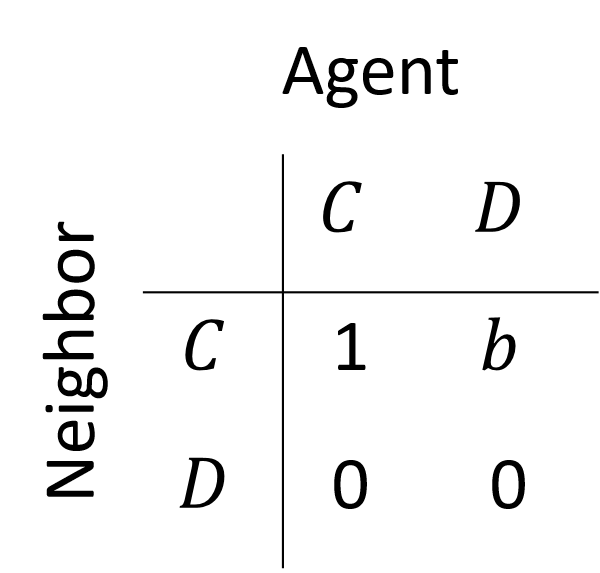
\includegraphics[width=0.22\textwidth]{Game_score_table.png}
\caption{The payoff matrix for a pairwise game. Setting the payoff of the
$\mathcal{C}$-$\mathcal{C}$ game does not limit generality, since it simply acts
to fix the payoff scale. This way, the only free parameter is $b$: the payoff of
a defector in a game with a cooperator. 
See text for discussion.}	
\label{fig:score-table}	
\end{center}
\end{figure}


The discrete structure of the payoffs implies that the dynamics of the game given
the initial conditions is insensitive to infinitesimal changes of the payoff parameter $b$ \cite{Nowak1992}.
The dynamics can only change at special values of $b$, which are nothing but simple fractions, $m/n$, 
where $m$ and $n$ are positive integers less then or equal to the number of elementary games of an agent.
On the square lattice this means that $1 \leqslant m, n \leqslant 9$ \cite{Nowak1992}. For the cubic lattice we consider in this work, 
%
\begin{equation}
1 \leqslant m, n \leqslant 27\;.
\label{mn}
\end{equation}


%%%%%%%%%%%%%%%%%%%%%%%%%%%%%%%%%%%%%%%%%%%%%%%%%%%%%%%%%%%%%%%%%%%%%%%%%%%%%%%
\section{Numerical simulations of the 3D game}
\label{sec:3D}

The original work Ref. \cite{Nowak1992, Nowak1993} and subsequent studies, \cite{Kolotev2018, Burovski2019},
investigated the game on a two-dimensional square and triangular lattices with $L\times L$ sites.
In this work, we use simple cubic lattice with $L\times L \times L$ sites.
Since we are ultimately interested in the behavior of the infinite population size, 
we use periodic boundary conditions to minimize finite-size effects.

%%%%%%%%%%%%%%%%%%%%%%%%%%%%%%%%%%%%%
\subsection{The steady-state behavior of the game}
\label{subsec:fc}

We simulate the game field with $L=60$ using 10 random realizations of initial conditions (replicas) at a fixed value of the initial concentration, $f_0 = 0.9$.
To reach the steady state, we monitor time dependence of the fraction of cooperators, $f_c$ (the number of cooperators divided by $L^3$). 
In most cases, $f_c$ stabilizes (up to fluctuations) in $\sim 2$-$3 \times 10^3$ time steps.  
We then simulate the game for $10^4$ steps and average over the time measurements and realizations of initial conditions.

Fig.\ \ref{fig:Fc} shows the dependence of the fraction of cooperators, $f_c$ on the payoff parameter $b$. 
For $b < 1$ the game converges to $f_c = 1$. For $b > 2$, the end state is $f_c = 0$. In the intermediate range, $1 < b < 2$, Fig.\ \ref{fig:Fc} clearly shows a non-monotonic behavior with large jumps at 
$b = 27 / n$, with $n\in\{1, 2, \ldots, 27\} $. This is due to the fact that for $b > 27/n$ isolated groups of $n$ or more defectors grow and convert their $\mathcal{C}$ neighbors into defectors.

\begin{figure}[H]
	\centering
	
	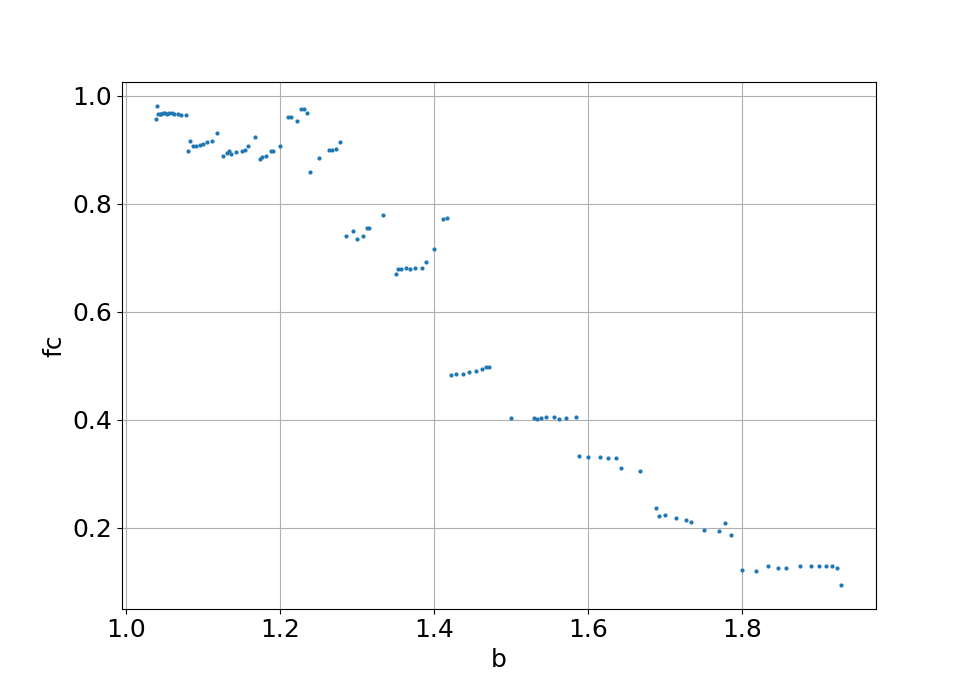
\includegraphics[width=0.5\textwidth]{C_0.9_graph.png}
	\caption{Average fraction cooperators as a function of the payoff parameter. Each point is the average of ten independent fields, with 100 measurements every 100 evolution steps.}
	\label{fig:Fc}
\end{figure}

\emph{Dependence on $f_0$.---} Since Fig.\ \ref{fig:Fc} shows a strong dependence on the payoff parameter, a natural question is what is the effect of the value of the initial concentration $f_0$. To this end we, perform similar simulations with
$f_0 = 0.1$ and $f_0 = 0.5$. For each value of $f_0$, we simulate 100 independent realizations of initial conditions at fixed $b$, and check the distribution of the steady state density $f_c$. Fig.\ \ref{fig:Fc0_hist} shows typical distributions. The distributions show well separated peaks: for smaller values of $f_0$, some replicas converge to the absorbing states $f_c = 0$ or $f_c = 1$. However, all other replicas converge to steady states with the average $f_c$ being independent of $f_0$. Furthermore, the number of replicas which converge to the absorbing states decreases with increasing $f_0$. We thus conclude that the results shown in Figure \ref{fig:Fc} are independent of $f_0$ once the replicas which converged to the absorbing states are discarded.


\begin{figure}[h]
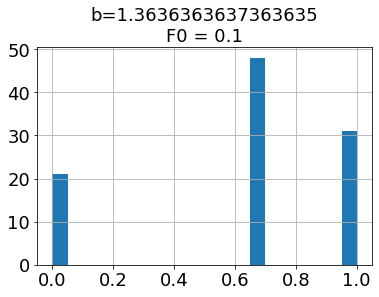
\includegraphics[width=0.3\textwidth]{b1,3_Fc0,1_hist.png} %
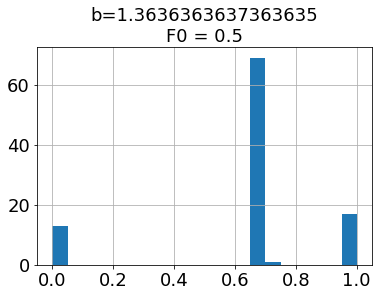
\includegraphics[width=0.3\textwidth]{b1,3_Fc0,5_hist.png} %
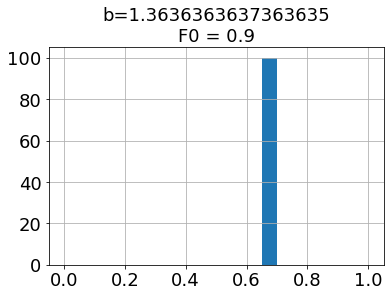
\includegraphics[width=0.3\textwidth]{b1,3_Fc0,9_hist.png}
%	
\caption{Histograms of the steady state $f_c$ for 100 independent realizations of initial conditions at $b\approx 1.3637$ and varying $f_0$. The values of $f_0$ are (from left to right) $0.1$, $0.5$ and $0.9$. Note that the central peak position is independent of $f_0$. the See text for discussion.}
\label{fig:Fc0_hist}
\end{figure}


\emph{Dependence on $L$.---} An important question is whether or not our results are affected by finite size effects. To this end, we performed simulations of the field size $100\times 100\times 100$ for a series of values of the payoff parameter $b$ and $f_0=0.9$. The steady state average density, $f_c$, is consistent for $L=60$ and $L=100$ within errorbars for all values of $b$. We thus conclude that $L=60$ simulations are representative of the thermodynamic limit $L\to\infty$.

%%%%%%%%%%%%%%%%%%%%%%%%%%%%%%%%%%%%%
\subsection{Spatial chaos}
\label{subsec:chaos}

To further chacterize the various steady state regimes, we investigate (i) how often an agent
changes the strategy, and (ii) what fraction of agents actually \emph{do} change
strategy at least once in the steady state. 
The latter quantity is known as the \emph{persistence} in the theory of disordered systems \cite{Bray1994, Majumdar1999}. Formally, perisistence $P(t_0, t_1)$ is the fraction of agents which did not change their stategy between time steps $t_0$ and $t_1$. In this work, we only study the steady state persistence, $P$, where both $t_0$ and $t_1$ are larger then the burn-in time and separated by $10^4$ time steps. Then $P=1$ means that the game field is completely static, and $P=0$ signals the chaotic regime where no agent keeps the strategy. 


\begin{figure}[H]
\begin{center}
	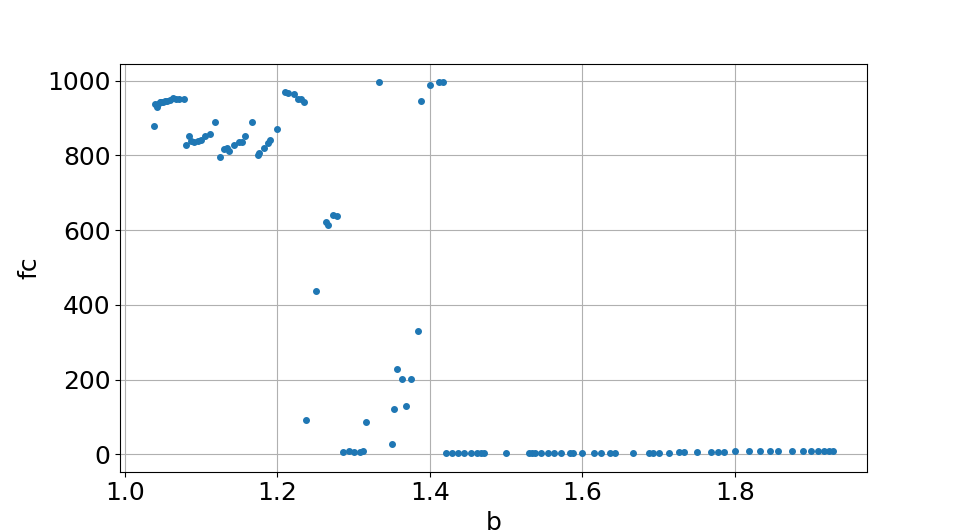
\includegraphics[width=0.55\textwidth, keepaspectratio=True]{Change_time.png} \\
%
	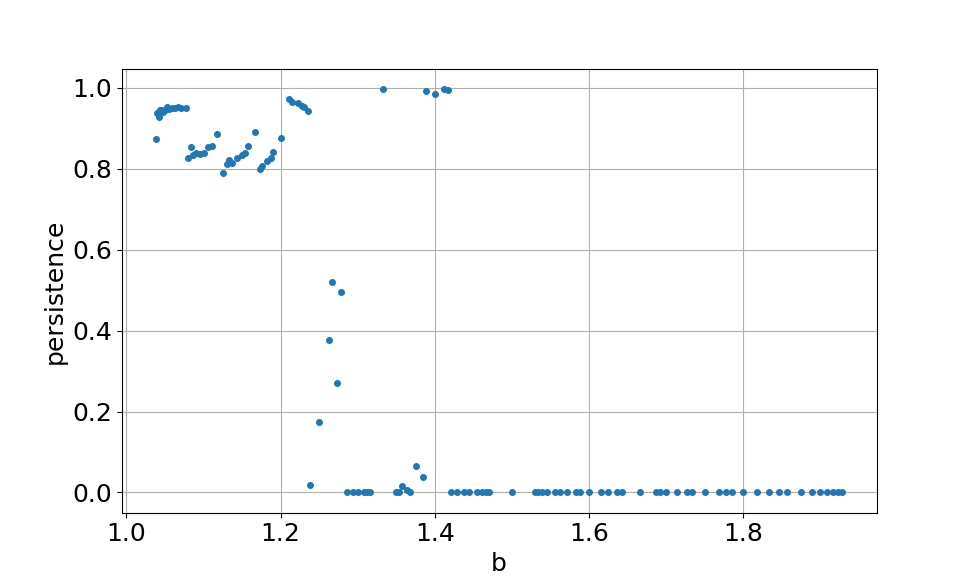
\includegraphics[width=0.55\textwidth, keepaspectratio=True]{Persistence.png}
	%
	\caption{(top panel) ``Mean switch time'': the average number of time steps for an agent to change their strategy as a function of the payoff parameter.  
	Points are simulation results averaged over all agents in a simulations of $10^{3}$ time steps for 10 realizations of initial conditions of the field with $L=60$ and $f_0 = 0.9$.
	(bottom panel) The steady-state persistence with $t_1 - t_0 = 10^4$ time steps. She simulations are done for 10 realizations of the initial conditions with $L=60$ and $f_0 = 0.9$. See text for discussion.
	}
	\label{fig:persistence}
\end{center}
\end{figure}


Fig.\ \ref{fig:persistence} shows simulation results for the mean time an agent keeps the strategy, $\tau_w$, and the steady state persistence, $P$. It is clear from Fig.\ \ref{fig:persistence} that $\tau_w$ and $P$ are
strongly correlated. For $b\in(1, 1.24)$,  $P$ and $\tau_w$ are almost proportional to each other and to the concentration of cooperators, cf. Fig.\ \ref{fig:Fc}. 
A possible explanation is that at these low values of $b$, defectors are separated in small isolated groups
and the boundaries of these clusters are ``blinking'': the agents at the boundaries are constantly changing their strategy back and forth. Therefore, the number of agents who change strategy is proportional to the number of defectors.  
For larger values of $b$, $b \approx 1.3$ we have $\tau_w \sim 1$ and $P\sim 0$, which signals the chaotic behavior: nearly all agents switch their strategies often. 

A striking feature of Fig.\ \ref{fig:persistence} is that the chaotic behavior is observed for a wide range of the payoff parameter $b$. This should be contrasted to the game on the square lattice, where the chaotic regime only covers $b\in (9/5, 2)$ and the triangular lattice, where the chaotic behavior is completely absent.


\section{Conclusions}

We study a model of spatially distributed evolutionary game based on the Prisoner's Dilemma. Using direct numerical simulations, we characterize the steady states of the game. Comparing our simulations of the game on the three-dimensional simple cubic lattice to two-dimensional simulations of \cite{Nowak1992, Nowak1993, Kolotev2018}, we find that the larger coordination number of the lattice facilitates the formation of spatial chaos. This way, the steady state of the game is chaotic in the large region of the payoff parameter.
The source code we used for simulations is available in Ref. \cite{github}. 

This research was supported in part through computational resources of HPC facilities at NRU HSE. L.~Shchur acknowledges the Scientific program of the Science Center of RAS in Chernogolovka.


\section*{References}
\begin{thebibliography}{9}

\bibitem{Axelrod2006} see, e.g., R.~Axelrod, \textit{The Evolution of Cooperation}, Basic Books,
2006, and references therein.

\bibitem{Smith1982} J. Maynard Smith, \textit{Evolution and the Theory of Games},
Cambridge University Press, (1982).

\bibitem{Nowak1992} M.A.~Nowak and R.M.~May, \textit{Evolutionary games
and spatial chaos}, Nature \textbf{359}, 826 (1992).

\bibitem{Nowak1993} M.A.~Nowak and R.M.~May, \textit{The spatial
dilemmas of evolution}, Int. J. Birurcation and Chaos \textbf{3}(1), 35-78 (1993).

\bibitem{Hauert2005} C.~Hauert and G.~Szabo, \textit{Game theory and physics},
Am. J. Phys. \textbf{73}(5), 405414 (2005).

%\bibitem{Hofbauer2008} see, e.g. J.~Hofbauer and K.~Sigmund, \textit{Evolutionary games and population dynamics}, Cambridge University Press, 2008.

\bibitem{Szolnoki2005} Gy\"{o}rgy Szab\'{o}, Jeromos Vukov, and Attila Szolnoki, \textit{Phase diagrams for an evolutionary prisoner’s dilemma game on two-dimensional lattices}, Phys. Rev. E \textbf{72}, 047107 (2005).

\bibitem{Szolnoki2017} Marco A. Amaral, Matjaz Perc,  Lucas Wardil, Attila Szolnoki, Elton J. da Silva J\'{u}nior, and Jafferson K. L. da Silva, \textit{Role-separating ordering in social dilemmas controlled by topological frustration}, Phys. Rev. E \textbf{95}, 032307 (2017).

\bibitem{Szolnoki2009} Attila Szolnoki and Matjaz Perc, \textit{Emergence of multilevel selection in the prisoner’sdilemma game on coevolving random networks}, New J. Phys. \textbf{11}, 093033 (2009).

\bibitem{Kolotev2018} S.~Kolotev, A.~Malyutin, E.~Burovski,~S. Krashakov, L.~Shchur, \textit{Dynamic fractals in spatial evolutionary games}, Physica A  \textbf{499}, 142 (2018)

\bibitem{Burovski2019} E.~Burovski, A.~Malyutin, L.~Shchur, \textit{On the geometric structures in evolutionary games on square and triangular lattices}, J. Phys.: Conf. Ser., \textbf{1290}, 012027 (2019) 

\bibitem{Arenzon2001}  Mendeli H. Vainstein and Jeferson J. Arenzon, \textit{Disordered environments in spatial games}, Phys Rev E \textbf{64}, 051905 (2001).

\bibitem{Bray1994} B. Derrida, A.J.~Bray, and G. Godr\'{e}che, J. Phys. A \textbf{27}, L357 (1994); A.J.~Bray, B.~Derrida, and G. Godr\'{e}che, Europhys. Lett. \textbf{27}, 175 (1994).

\bibitem{Majumdar1999} S.N.~Majumdar, Curr. Sci. \textbf{77}, 370 (1999).

\bibitem{github} https://github.com/MoskalenkoRomanBorisovich/Spatial-Distribution-Evolutionary-Game 


\end{thebibliography}

\end{document}
